% $Id$

\documentclass[a4paper,12pt]{article}

\usepackage{graphicx}

\setlength{\parindent}{0mm}
\setlength{\parskip}{7.5mm}

\begin{document}

\title{4ICT9 \\ Assignment 2 \\ Network Planning Laboratory}

\author{David Collins 02704030 \\ collinda@tcd.ie \\ 
Conall O'Brien 01734351 \\ conallob@maths.tcd.ie}

\maketitle

\section{Group Tasks}

The assignment was broken down in the following structure

\begin{tabular}{lcl}
Entire Group &	\hspace{15mm}	&	Descision on Geographical Location	\\
David Collins	&					&	Construction of Composite Map			\\
Conall O'Brien	&					&	Mapping of Mobile Network and Routes\\
David Collins	&					&	Simulation of Routes around Network	\\
Conall O'Brien	&					&	Preparation of Report					\\
\end{tabular}

\section{Geographic Location Chosen}

Our group decided to create a mobile network in Amsterdam, The
Netherlands.

\subsection{Reasons Why}

There are two reason our group decided to creatge a network in
Amsterdam.


The first reason is in regard to the general consensus is that 
Amsterdam, like much of The Netherlands, has benefitted from impressive
town planning, design and layout for centuries. Amsterdam has a very 
dense, urban centre, surrounded by urban sectors filled with town houses
used as apartments. In addition, modern building developemnts are often
done on reclaimed land near the city centre. Further away from the city
centre are more traditional suburban sectors including public green
spaces such as parks. The various dense urban, urban and suburban areas
are all partitioned from each other using significant landmarks such as
canals or major roads.


The second reason why Amsterdam was chosen was first hand knowledge. One
of the members of our group recently visited Amsteram, thus enabling him
to derive many routes between landmarks, tourist attractions and various
areas of Amsterdam, with the intention of simulating them on the mobile
network.

\subsection{Map}


\begin{figure}[h]

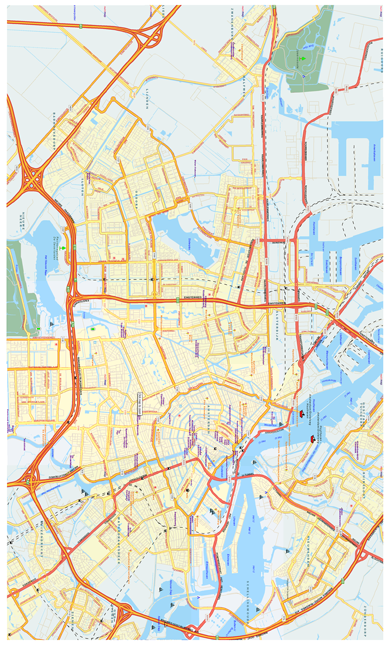
\includegraphics{amsterdam.png}

\caption{Composite Map before Defining Areas and Mapping Routes}

\end{figure}

\pagebreak

\begin{figure}[h]

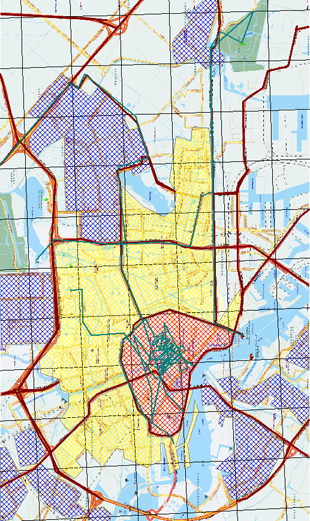
\includegraphics{routes.png}

\caption{Overview of map with Areas and Mobile Routes defined}

\end{figure}

\section{Simulation Results}

\begin{figure}[h]

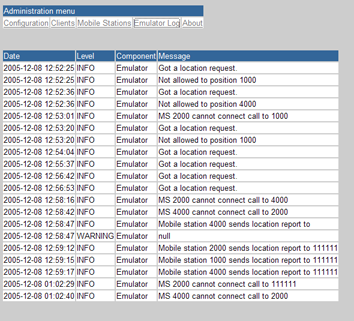
\includegraphics{screen7.png}

\caption{General Simulation Overview}

\end{figure}


\section{Problems Encountered}

While attempting to plan the mobile network, Conall repeatidly
encoutered unusual behaviour with the Eircsson Mapping Tool. While
importing a map and specifying specific Latitude and Longitude values
for a reference point on the map, Latitude and Longitude kept appearing
erroniously as shown in figure 8. To solve this problem, Conall
was advices to set the width of the map to 140km after inputting the 
Latitude and Longitude for the map. 

\begin{figure}[h]

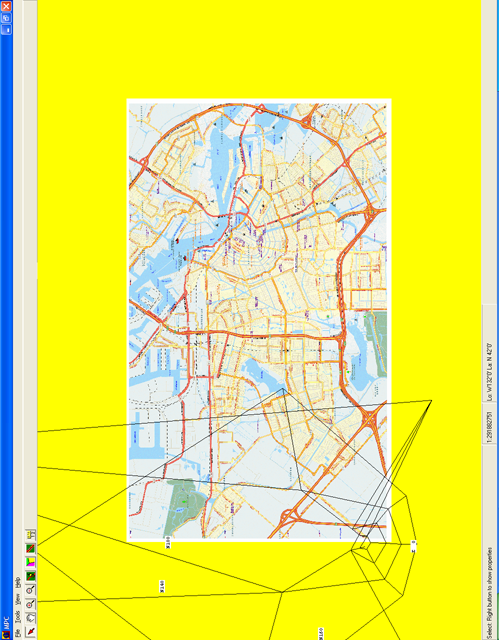
\includegraphics{oddness.png}

\caption{Mapping Tool Problem Encountered}

\end{figure}

When attempting to simulate the 4 mobile phone routes, mobile route 3000
did not appear in the simulator. Despite being defined in the Mapping
Tool, we were unable to explain why it did not simulate.

\end{document}
